\documentclass[man]{apa6}
\usepackage{lmodern}
\usepackage{amssymb,amsmath}
\usepackage{ifxetex,ifluatex}
\usepackage{fixltx2e} % provides \textsubscript
\ifnum 0\ifxetex 1\fi\ifluatex 1\fi=0 % if pdftex
  \usepackage[T1]{fontenc}
  \usepackage[utf8]{inputenc}
\else % if luatex or xelatex
  \ifxetex
    \usepackage{mathspec}
  \else
    \usepackage{fontspec}
  \fi
  \defaultfontfeatures{Ligatures=TeX,Scale=MatchLowercase}
\fi
% use upquote if available, for straight quotes in verbatim environments
\IfFileExists{upquote.sty}{\usepackage{upquote}}{}
% use microtype if available
\IfFileExists{microtype.sty}{%
\usepackage{microtype}
\UseMicrotypeSet[protrusion]{basicmath} % disable protrusion for tt fonts
}{}
\usepackage{hyperref}
\hypersetup{unicode=true,
            pdftitle={Objectification in Action: Self- and Other-Objectification in Same-gender Interactions},
            pdfauthor={Randi L. Garcia, Kat Kyuchukova, \& Asha Hinson},
            pdfkeywords={keywords},
            pdfborder={0 0 0},
            breaklinks=true}
\urlstyle{same}  % don't use monospace font for urls
\usepackage{graphicx,grffile}
\makeatletter
\def\maxwidth{\ifdim\Gin@nat@width>\linewidth\linewidth\else\Gin@nat@width\fi}
\def\maxheight{\ifdim\Gin@nat@height>\textheight\textheight\else\Gin@nat@height\fi}
\makeatother
% Scale images if necessary, so that they will not overflow the page
% margins by default, and it is still possible to overwrite the defaults
% using explicit options in \includegraphics[width, height, ...]{}
\setkeys{Gin}{width=\maxwidth,height=\maxheight,keepaspectratio}
\IfFileExists{parskip.sty}{%
\usepackage{parskip}
}{% else
\setlength{\parindent}{0pt}
\setlength{\parskip}{6pt plus 2pt minus 1pt}
}
\setlength{\emergencystretch}{3em}  % prevent overfull lines
\providecommand{\tightlist}{%
  \setlength{\itemsep}{0pt}\setlength{\parskip}{0pt}}
\setcounter{secnumdepth}{0}
% Redefines (sub)paragraphs to behave more like sections
\ifx\paragraph\undefined\else
\let\oldparagraph\paragraph
\renewcommand{\paragraph}[1]{\oldparagraph{#1}\mbox{}}
\fi
\ifx\subparagraph\undefined\else
\let\oldsubparagraph\subparagraph
\renewcommand{\subparagraph}[1]{\oldsubparagraph{#1}\mbox{}}
\fi

%%% Use protect on footnotes to avoid problems with footnotes in titles
\let\rmarkdownfootnote\footnote%
\def\footnote{\protect\rmarkdownfootnote}


  \title{Objectification in Action: Self- and Other-Objectification in
Same-gender Interactions}
    \author{Randi L. Garcia\textsuperscript{1, 2}, Kat
Kyuchukova\textsuperscript{1}, \& Asha Hinson\textsuperscript{1}}
    \date{}
  
\shorttitle{Objectification in Action}
\affiliation{
\vspace{0.5cm}
\textsuperscript{1} Department of Psychology, Smith College\\\textsuperscript{2} Program in Statistical and Data Sciences, Smith College}
\keywords{keywords}
\usepackage{csquotes}
\usepackage{upgreek}
\captionsetup{font=singlespacing,justification=justified}

\usepackage{longtable}
\usepackage{lscape}
\usepackage{multirow}
\usepackage{tabularx}
\usepackage[flushleft]{threeparttable}
\usepackage{threeparttablex}

\newenvironment{lltable}{\begin{landscape}\begin{center}\begin{ThreePartTable}}{\end{ThreePartTable}\end{center}\end{landscape}}

\makeatletter
\newcommand\LastLTentrywidth{1em}
\newlength\longtablewidth
\setlength{\longtablewidth}{1in}
\newcommand{\getlongtablewidth}{\begingroup \ifcsname LT@\roman{LT@tables}\endcsname \global\longtablewidth=0pt \renewcommand{\LT@entry}[2]{\global\advance\longtablewidth by ##2\relax\gdef\LastLTentrywidth{##2}}\@nameuse{LT@\roman{LT@tables}} \fi \endgroup}


\DeclareDelayedFloatFlavor{ThreePartTable}{table}
\DeclareDelayedFloatFlavor{lltable}{table}
\DeclareDelayedFloatFlavor*{longtable}{table}
\makeatletter
\renewcommand{\efloat@iwrite}[1]{\immediate\expandafter\protected@write\csname efloat@post#1\endcsname{}}
\makeatother

\authornote{

Correspondence concerning this article should be addressed to Randi L.
Garcia, 415 Bass Hall, Smith College, Northampton, MA 01060. E-mail:
\href{mailto:rgarcia@smith.edu}{\nolinkurl{rgarcia@smith.edu}}}

\abstract{
Empirical evidence has only found links between objectification,
self-objectification, and negative outcomes for woman within
interpersonal interactions between male-female pairs. The purpose of the
present study was to extend past research and consider the relationships
between such valuable phenomena and their effects on authenticity within
interactions between female pairs. Woman were brought into the
laboratory and interacted in same-sex dyads. Dyadic analysis was
utilized to detect whether partners' objectification of each other
affected state self-objectification, and the resulting feelings of
comfort and authenticity during the interaction. After the interaction,
participants completed a questionnaire which measured many constructs
including cognitive performance, career aspirations, and relationship
agency. Results revealed no significant relationship between
self-objectification and authenticity. Further, although there were
significantly negative effects on career aspirations and relationship
agency resulting from a lack of relationship authenticity, there was no
evidence that this is due to feelings of sexual objectification. The
significant partner effect of objectification on actor
self-objectification suggests that women being objectified by other
women still results in feelings of self-objectification, and such
research has powerful implications for the ways that women interact in
both sexual and non-sexual settings. AUTHOR NOTE: mention Clark trigram
coders Hannah et al.


}

\begin{document}
\maketitle

Theorists across diverse disciplines have explored the multiple ways
that the body conveys social meaning, as well as how these meanings
shape gendered experiences, especially during interpersonal interactions
with members of different social groups (``Engendered lives,'' 1993,
Garcia, Earnshaw, and Quinn (2016)). Objectification theory, a valuable
theoretical framework proposed by Roberts and Fredrickson (1997) which
works to contextualize female bodies as socio-cultural constructions,
can be employed to illuminate the gender oppression and negative lived
experiences of girls and women. Empirical evidence illustrates how women
continue to be objects of interpersonal discrimination and expereince
daily sexist hassles (Swim, Hyers, Cohen, \& Ferguson, 2001). One form
of interpersonal discrimination women face is the process by which their
whole being is viewed as a collection of sexualized body parts valued
predominantly for commodification, a phenomena termed sexual
objectification (Bartky, 1990). Sexual objectification occurs with both
\enquote{endless variety and monotonous similarity,} and is thus
mediated by unique combinations of race, ethnicity, sexuality, age, and
class (Fredrickson, Hendler, Nilsen, O'Barr, \& Roberts, 2011; Rubin,
1975, cited in Fraser and Nicholson (1989), p.~28). Amid such
heterogeneity though, \enquote{having a reproductively mature female
body} proposed by Roberts and Fredrickson (1997) is likely to create a
shared vulnerability to sexual objectification and a variety of shared
negative experiences as a result.

Self-objectification is a multidimensional process that accounts for the
cognitive mechanism that translates experiences of sexualization at the
cultural level to psychological (e.g., anxiety, self-esteem,
authenticity, motivational states) and behavioral (cognitive
performance, body monitoring) features of mental health and well-being
at the individual level (Calogero, Tantleff-Dunn, \& Thompson, 2011;
Moradi \& Huang, 2008). Calogero et al. (2011) proposes that the
construct of self-objectification can be conceptualized as a learned
trait. Furthermore, it can also be elicited momentarily, through the
media, for example, with sexualized images in movies and magazines,
which can lead to a state of self-objectification (Calogero et al.,
2011, Moradi and Huang (2008)). Being objectified by another person and
possessing trait-level self-objectification (TSO) may interact to
influence experiences of feeling like a body, or state
self-objectification (SSO) (CITE swimsuit sweater, Garcia et al., 2016).

Studies have shown that within social encounters women are gazed at more
than men (Briton \& Hall, 1995, CITE saguy skype study, calogero video
walking study), often times feel \enquote{looked at} within
interpersonal interactions (Argyle \& Williams, 1969), and will more
than likely internalize the objectifying gaze on physical self (Young,
1979). Moreover, perhaps the most adverse effect of objectifying
treatment is that it effectively socializes girls and women to treat
themselves as objects to be looked at and evaluated, an effect termed
self-objectification (Bartky, 1990; Berger, Cohen, \& Zelditch Jr, 1972;
L. Fredrickson, Roberts, M. Noll, Quinn, \& Twenge, 1998).

ENTIRE PARAGRAPH ON MODERN (POST-2016) STUDIES OF INTERPERSONAL
OBJECTIFICATION.

Empirical evidence reveals that objectification manifests through
inauthenticity in romantic relationships (Brunell et al., 2010), adverse
attitudes in regard to career aspirations, and a decrease in
concentration and impairment in female cognitive performance (D. M.
Quinn, Chaudoir, \& Kallen, 2011).

In the current study, we sought to examine what occurs during an
interaction in which one or both partners are objectifying each other,
similarly to Garcia et al. (2016), but between same-sex female
interpersonal interactions. Moreover, the current study uses a
face-to-face interaction paradigm and dyadic data analysis techniques to
examine the effects for both women simultaneously. We expected to
replicate the results found in Garcia et al. (2016). We predicted that
being objectified by one's interaction partner would lead to
self-objectification, which in turn would lead to feelings of
inauthenticity, then reduced feelings of agency in romantic
relationships, reduced career aspiration, and reduced cognitive
performance. Specifically, we expected to find a positive relationship
between other-objectification by one's partner and state
self-objectification. We also expect to find a negative relationship
between self-state objectification and interaction authenticity, and
that interaction authenticity will be positively related to cognitive
performance, relationship agency, and career aspirations.

\section{Methods}\label{methods}

\subsection{Procedure}\label{procedure}

The procedure used was identical to that in Garcia et al. (2016), except
for the instructions that the participants were given. In brief, that
methodology is that each participant arrived at the laboratory and were
then led into separate cubicles to prevent any communication between the
participants before the interaction. In addition, each participant was
screened for prior acquaintance to confirm that they had not met prior
to the study. They were asked to sign the consent form to participate,
and the study was described as follows: \enquote{This is a study looking
at how students form different types of relationships at college.} A
prompt on the computer screen told the participants that they were
assigned to the \enquote{College Relationships} condition and gave the
following instructions:

There are many types of relationships people form in college. During the
interaction, please think about your partner's potential as a romantic
partner. Even if they are not the gender you are attracted to, you can
still judge their potential as a romantic partner. After the interaction
you will be asked to evaluate how dateable your partner is. In other
words, we would like to know if you think someone would date your
interaction partner. Also, your interaction partner will be evaluating
you in the same manner.

Two participants were then brought into a larger interaction room where
they sat on stools prearranged to be 36 inches apart. The experimenter
instructed the participants to \enquote{get to know each other} for 10
minutes and then left the room. After 10 minutes, the experimenter came
back into the room and stopped the interaction. The participants then
went back to their individual cubicles and completed a set of
post-interaction measures. Participants were then thanked for their
participation and debriefed Garcia et al. (2016). The full methodology
used is found in Garcia et al. (2016)'s study.

\subsection{Combined Samples}\label{combined-samples}

Data from two different, but demographically equivalent, samples were
combined to create the final analysis sample (\emph{N =} 64) used in
this study. In the measures section that follows we refer to them as
Sample 1 and Sample 2. Sample 1 (\emph{N =} 24) is from a co-ed liberal
arts college in the northeast US and Sample 2 (\emph{N =} 40) is from a
women's liberal arts college in the northeast US. The description of the
samples section below contains more detail about equivalence analyses to
support the decision to combine these two samples.

\subsection{Post interaction Measures}\label{post-interaction-measures}

\begin{table}[tbp]
\begin{center}
\begin{threeparttable}
\caption{\label{tab:corrtable}Correlations among study variables.}
\begin{tabular}{llllllll}
\toprule
 & \multicolumn{1}{c}{$M$} & \multicolumn{1}{c}{$SD$} & \multicolumn{1}{c}{1} & \multicolumn{1}{c}{2} & \multicolumn{1}{c}{3} & \multicolumn{1}{c}{4} & \multicolumn{1}{c}{5}\\
\midrule
Actor's trait self objectification (TSO) & -0.35 & 2.64 &  &  &  &  & \\
Actor's authenticity of interaction & 5.23 & 1.02 & -.02 &  &  &  & \\
Actor's objectification of partner & -1.58 & 1.21 & .20 & -.07 &  &  & \\
Actor's state self-objectification & 1.92 & 1.13 & .13 & -.10 & -.09 &  & \\
Actor's future relationship agency & 4.69 & 0.96 & .04 & .23+ & .09 & -.09 & \\
Actor's cognitive performance & 5.03 & 2.29 & .08 & .11 & .11 & .02 & .07\\
\bottomrule
\end{tabular}
\end{threeparttable}
\end{center}
\end{table}

\begin{table}[tbp]
\begin{center}
\begin{threeparttable}
\caption{\label{tab:descriptives}Descriptive Statistics for Study Variables}
\begin{tabular}{lll}
\toprule
 & \multicolumn{1}{c}{M} & \multicolumn{1}{c}{SD}\\
\midrule
Actor's trait self objectification (TSO) & -0.35 & 2.64\\
Actor's authenticity of interaction & 5.23 & 1.02\\
Actor's objectification of partner & -1.58 & 1.21\\
Actor's state self-objectification & 1.92 & 1.13\\
Actor's future relationship agency & 4.69 & 0.96\\
Actor's cognitive performance & 5.03 & 2.29\\
\bottomrule
\end{tabular}
\end{threeparttable}
\end{center}
\end{table}

The following measures were collected in the order they are presented
following the interaction. Correlations appear in
Table~\ref{tab:corrtable}, and descriptive statistics appear in
Table~\ref{tab:descriptives}.

\subsubsection{Cognitive Performance}\label{cognitive-performance}

Trigrams from the Remote Associates Task (McFarlin \& Blascovich, 1984)
were utilized to assess cognitive performance after the interaction. Ten
items were selected and presented to participants. For example, the
correct answer for the trigram \enquote{Quack: Pond: Waddle} would be
\enquote{Duck}. Participants are limited to 30 seconds. For every
correct answer, 1 point is given. The mean score was 5.03 (SD = 2.29).
Cognitive performance was measured first in order to measure potential
immediate detriments to performance (Garcia et al., 2016).

\subsubsection{State
Other-Objectification}\label{state-other-objectification}

To measure the participant's objectification of their partner in the
interaction, participants were asked a series of questions about the
frequency of thoughts in relation to multiple characteristics of their
partner Garcia et al. (2016). Questions included aspects of their
partner's internal traits such as personality, friends, family, and
extracurricular interests, as well as external traits such as body,
appearance, clothing, and body parts. All questions were to be rated on
a scale from 1 (not at all) to 7 (constantly). Objectification was
measured by getting the difference between the average frequency of
thought about their partner's external traits (\(\alpha\) = 0.79 for
Sample 1, \(\alpha\) = 0.79 for Sample 2) and frequency of thought about
their partner's internal traits (\(\alpha\) = 0.79 for Sample 1,
\(\alpha\) = 0.76 for Sample 2). A positive score in this scale would
indicate that the participant thought about their partner's external
traits more than the partner's internal traits, and a negative score
would indicate the opposite.

\subsubsection{Interaction Authenticity}\label{interaction-authenticity}

To assess the magnitude to which individuals felt comfortable in the
interaction and perceived the interaction to be authentic, we asked
participants to rate the extent to which they felt comfortable, happy,
friendly, warm, easygoing, sincere, and authentic on a scale ranging
from 1 (not at all) to 7 (very much), much alike (Garcia et al., 2016).
Participants were additionally asked to rate their interaction partner's
authenticity as well as their own: \enquote{`Do you think your partner
was authentic during your interaction?}' and \enquote{`Were you
authentic during your interaction?}' These questions were ranked on a
scale from 1 (not authentic at all). These were combined to form the
authenticity scale (\(\alpha\) = 0.91 for Sample 1, \(\alpha\) = 0.91
for Sample 2).

\subsubsection{State
Self-Objectification}\label{state-self-objectification}

To assess state self-objectification, we used an average of two items
from Saguy, Quinn, F Dovidio, and Pratto (2010) that were also used in
Garcia et al. (2016). Participants were asked to rank how much they
agreed with the following statements: \enquote{During the interaction I
felt more like a body than a full self} and \enquote{I felt more like a
body than as a real person in the interaction}. Originally, Saguy et al.
(2010) used 3 items, but in both samples the reliability of the scale
was higher once the third item was removed, so we chose to only use the
first two for our measure of SSO, leaving us with a reliable scale
(\(\alpha\) = 0.84 for Sample 1, and \(\alpha\) = 0.85 for Sample 2.)

\subsubsection{Relationship Agency}\label{relationship-agency}

A scale was used from Garcia et al. (2016) to assess how much agency an
individual believes they would possess in future romantic relationships.
Participants were asked how likely it was that they would do the
following: \enquote{`ask someone out on a date,}' \enquote{`open the
door for your date,}' \enquote{`pay for a date,}' \enquote{`ask your
boyfriend/girlfriend to marry you,}' \enquote{`initiate sex with your
girlfriend/boyfriend,}' \enquote{`initiate condom use during sex,}'
\enquote{`surprise your boyfriend/ girlfriend with a gift,}' and
\enquote{`ask your girlfriend/boyfriend to move with you to a new
place.}' Responses were measured on a scale ranging from 1 (not at all
likely) to 7 (extremely likely). The scale originally had 9 items, but
the 9th item had low correlations with the remaining items, ranging from
.02 to .30 for the first sample, and .04 to .30 for the second sample.
The item was intended to be reverse coded, but correlations were still
low enough to make the scale unreliable. Therefore, the ninth item was
removed. As a result, the scale had moderately high reliability for both
samples (\(\alpha\) = 0.72 for Sample 1, (\(\alpha\) = 0.74 for Sample
2).

\subsubsection{Career Aspirations}\label{career-aspirations}

To conceptualize participants' career aspirations after the interaction,
we used the 10-item adaptation of P. Gray and M. OBrien (2007)'s Career
Aspiration Scale employed in Garcia et al. (2016), which asked
participants to consider how true 10 statements were in regard to their
future careers on a scale from 0 (not at all true of me) to 4 (very true
of me). Items include \enquote{I hope to become a leader in my career
field} and \enquote{I hope to move up through any organization or
business I work in.} Items were fairly reliable (\(\alpha\) = 0.73 for
Sample 1, \(\alpha\) = 0.80 for Sample 2).

\subsubsection{Trait
Self-Objectification}\label{trait-self-objectification}

Trait self-objectification (TSO) was assessed using the
Self-Objectification Questionnaire (L. Fredrickson et al., 1998; M. Noll
\& L. Fredrickson, 1998), which evaluates the extent to which
individuals view their bodies in observable versus nonobservable ways.
The questionnaire asked participants to rank order both appearance and
functional aspects of their bodies, from 1 (least important) to 10 (most
important), with respect to physical self-concepts. Of the ten body
attributes, five of the items were appearance-based (weight, sex appeal,
physical attractiveness, firm/sculpted muscles and body measurements),
and five of the items were competence-based (strength, physical
coordination, energy level, health and physical fitness). Difference
scores were computed by subtracting the sum of the 5 functional
aspects/competence attributes (e.g., health, strength) from the sum of
the 5 physical self-concepts/appearance attributes (e.g., physical
attractiveness, weight), and all measures were multiplied by -1, as was
done in Garcia et al. (2016), so that positive scores indicated greater
TSO.

\subsubsection{Description of the
Samples}\label{description-of-the-samples}

Thirty-two previously unacquainted self-identifying female-sex dyads (64
total participants) from two liberal arts institutions in the Northeast
of the United States participated in this study. More specifically,
twelve of the pairs, which derived from Sample 1, were students at a
co-ed liberal arts college, while the remaining twenty pairs who came
from Sample 2 attended a women's liberal arts college. Initially, data
was collected from same-sex and mixed-sex dyads that comprised of male
and female gendered individuals. Sample 1 originally consisted of
twenty-two pairs, twelve men and thirty-two women. Twenty-three pairs
made up of forty-three women and one man, as well as two participants
who did not identify with either gender category, formed Sample 2. For
consistency, we limited participant data to same sex female pairs at the
two colleges.

Due these similarities across samples in regard to correlation patterns
between significant variables within this study, the two datasets were
combined. These participants were mostly first-year college students,
with an average age of 18.85 (SD = 1.04). The sample was 48.44\%
White/European American, 9.38\% Black/African-American, 28.12\%
Asian/Pacific Islander, 9.38\% Latinx, and 4.69\% mixed-race. There were
8 White/White pairs and 4 same race racial minority pairs, for a total
of 12 same-race pairs. The remaining 20 were mixed race pairs, of which
15 were White/racial minority pairings and 5 were cross-racial minority
group pairs. 64.06\% of the sample identified as heterosexual, and 25\%
identified as gay, lesbian or bisexual.

\section{Results}\label{results}

\subsection{Data analysis}\label{data-analysis}

We used R (Version 3.5.2; R Core Team, 2017) and the R-packages
\emph{apaTables} (Version 2.0.5; Stanley, 2018), \emph{devtools}
(Version 1.13.5; Wickham, Hester, \& Chang, 2018), \emph{dplyr} (Version
0.8.3; Wickham, François, Henry, \& Müller, 2018), \emph{forcats}
(Version 0.3.0; Wickham, 2018), \emph{ggformula} (Version 0.7.0; D.
Kaplan \& Pruim, 2017), \emph{ggplot2} (Version 3.2.1; Wickham, 2016),
\emph{haven} (Version 2.1.0; Wickham \& Miller, 2019), \emph{irr}
(Version 0.84.1; Gamer, Lemon, \&
\textless{}puspendra.pusp22@gmail.com\textgreater{}, 2012), \emph{knitr}
(Version 1.25; Xie, 2015), \emph{kutils} (Version 1.70; Johnson, Kite,
\& Redmon, 2019), \emph{lattice} (Version 0.20.38; Sarkar, 2008),
\emph{lavaan} (Version 0.6.1; Rosseel, 2012), \emph{lpSolve} (Version
5.6.15; Berkelaar \& others, 2015), \emph{Matrix} (Version 1.2.15; Bates
\& Maechler, 2017), \emph{mosaic} (Version 1.2.0; Pruim, Kaplan, \&
Horton, 2017, 2016), \emph{mosaicData} (Version 0.17.0; Pruim et al.,
2016), \emph{nlme} (Version 3.1.137; Pinheiro, Bates, DebRoy, Sarkar, \&
R Core Team, 2017), \emph{papaja} (Version 0.1.0.9842; Aust \& Barth,
2018), \emph{psych} (Version 1.8.4; Revelle, 2017), \emph{purrr}
(Version 0.3.2; Henry \& Wickham, 2019), \emph{readr} (Version 1.1.1;
Wickham, Hester, \& Francois, 2017), \emph{stringr} (Version 1.4.0;
Wickham, 2019), \emph{tibble} (Version 2.1.3; Müller \& Wickham, 2019),
\emph{tidyr} (Version 1.0.0; Wickham \& Henry, 2019), \emph{tidyverse}
(Version 1.2.1; Wickham, 2017), \emph{usethis} (Wickham \& Bryan, 2018),
and \emph{xtable} (Version 1.8.3; Dahl, Scott, Roosen, Magnusson, \&
Swinton, 2019) for all our analyses.

\subsection{Analysis Strategy}\label{analysis-strategy}

\begin{figure}
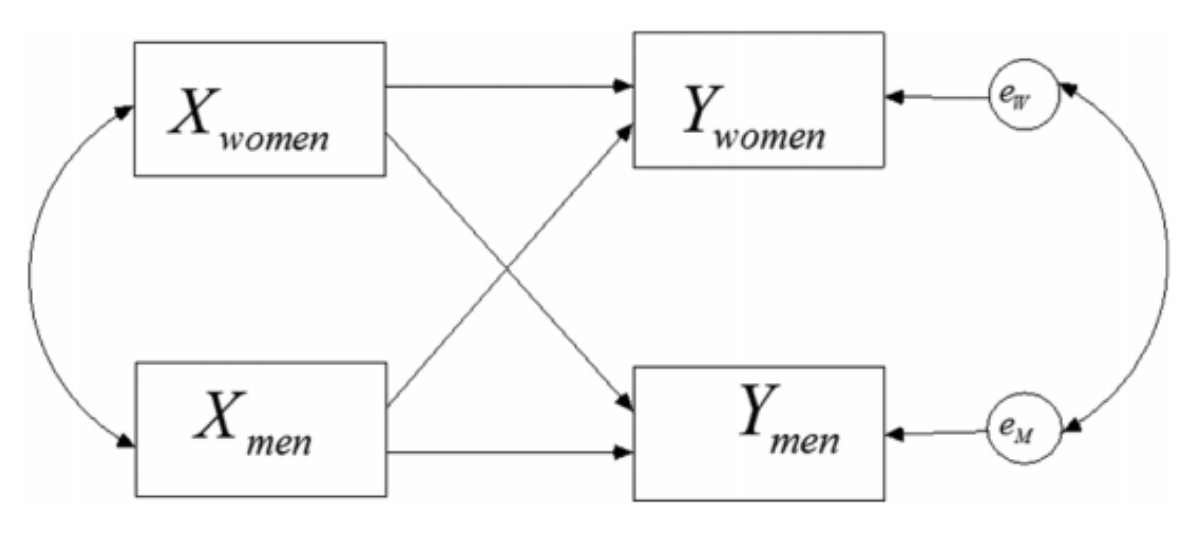
\includegraphics[width=400px]{APIM_figure} \caption{Basic actor-partner interdependence model (APIM) depiction.}\label{fig:apim}
\end{figure}

\begin{figure}
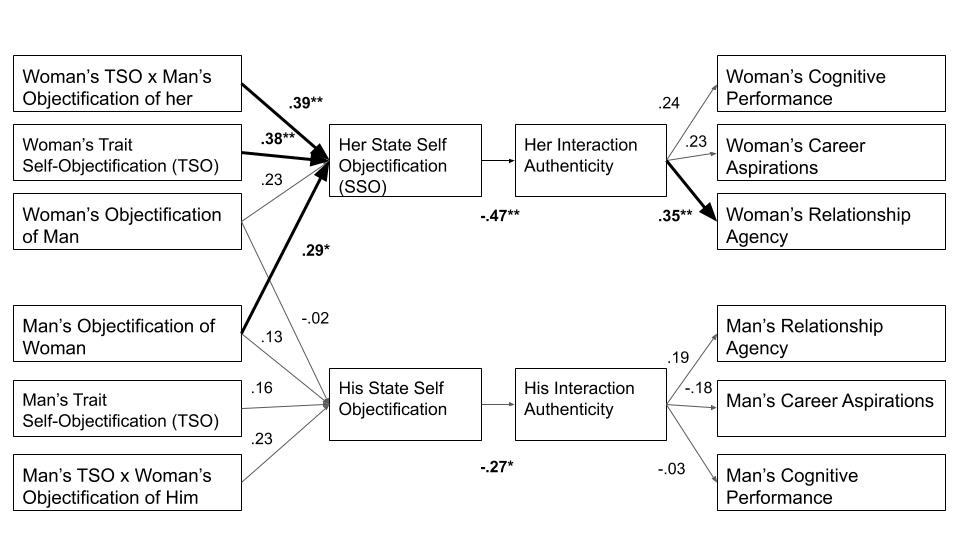
\includegraphics[width=400px]{2016_figure} \caption{Path Analysis Model from Garcia et al. (2016) study with distinguishable dyads.}\label{fig:2016figure}
\end{figure}

This study sought to replicate the results of Garcia et al. (2016)'s
study, done with male-female pairs, which used a dyadic path analysis to
detect whether partners' objectification of one another affected state
self-objectification (SSO). See Figure~\ref{fig:2016figure} for the
results of the analysis from this previous study. We hope to investigate
how the central effects found in the previous study relate to
interactions between two women. Specifically, we are interested in
testing the relationship between state-other objectification and SSO,
and how SSO in turn, affecs feelings of inauthenticity during the
interaction. In addition, we will also test if the effect of
other-objectification in an interaction on SSO is only present for those
women who are high in trait self-objectification, as in Garcia et al.
(2016). Further, we will investigate the realtionships between
experiencing interaction inauthenticity and relationship agency, career
aspirations, and cognitive performance.

While Garcia et al. (2016) used dyadic path analysis, we will conduct
our dyadic analyses using multilevel modeling. Dyadic analyses for
distingishable dyads (e.g., mixed-gender interacting pairs) is more
natural in Structual Equation Modeling (SEM) than it is for
indistinguishable dayds (e.g., same-gender interacting pairs) (Garcia,
Kenny, \& Ledermann, 2015; Ledermann \& Kenny, 2017). One reason for
this asymmetry is that, due to the arbitrary distinctions made bewteen
\enquote{partner 1} and \enquote{partner 2} in indistinguishable dyads,
many estimates need to be fixed to be equal (i.e., paths, variances,
covariances, endogenous intercepts, and exogenous means) for
indistinguishable dyads but these equality contraints should not then be
considered in the degrees of freedom calculations for fit estimations
(Olsen \& Kenny, 2006). Further, Olsen and Kenny (2006) detail how a new
independence model and the corresponding fit measure should be
re-calculated for indistinguishable dyads models. The current study uses
dyadic multilevel modeling (MLM) to test all relationships and mediation
paterns. See Ledermann and Kenny (2017) for a more complete discussion
of the considerations for using SEM versus MLM for dyadic analysis.

Testing the Garcia et al. (2016) model on the current, same-gender,
sample, involves using the Actor-Partner Independence Model (APIM)
approch for each outcome variable (i.e., endogenous variable in
Figure~\ref{fig:2016figure}). Thus, we ran five APIM's to test all the
hypothesized relationships. See Figure~\ref{fig:apim} for a basic APIM
model. The APIM includes effects due to one's own, as well as one's
partner's, predictor variables (\(X\)'s) on the one's own outcome
variable (\(Y\)). Unlike the original Garcia et al. (2016) study, our
study deals with indistinguishable dyads, meaning the designation of who
is designated as \enquote{actor} and who is designated as
\enquote{partner} is arbitrary. Recall that the indistinguiahble nature
of the dyads in the current study led us to choose the MLM approach over
SEM. These analyses are considered exploratory, given the lack of prior
research theorizing about these linkages.

Before moving to the main analyses, we discuss statistical equivalence
test that provide support for combining Sample 1 and Sample 2 in one
analysis sample. The online supplemental material contains the main
analyses separated by samples.

\subsubsection{Combining Samples}\label{combining-samples}

The correaltions between study variables is similar across samples. The
realibialities for the study scales were also equivalent. (Note that the
two samples were two small to conduct formal measurement equivalence
tests for scales.) There are no statistically significant differences
between samples in demographics including age, STATS, and ethnicity,
STATS.

\subsection{Main Results}\label{main-results}

\begin{figure}
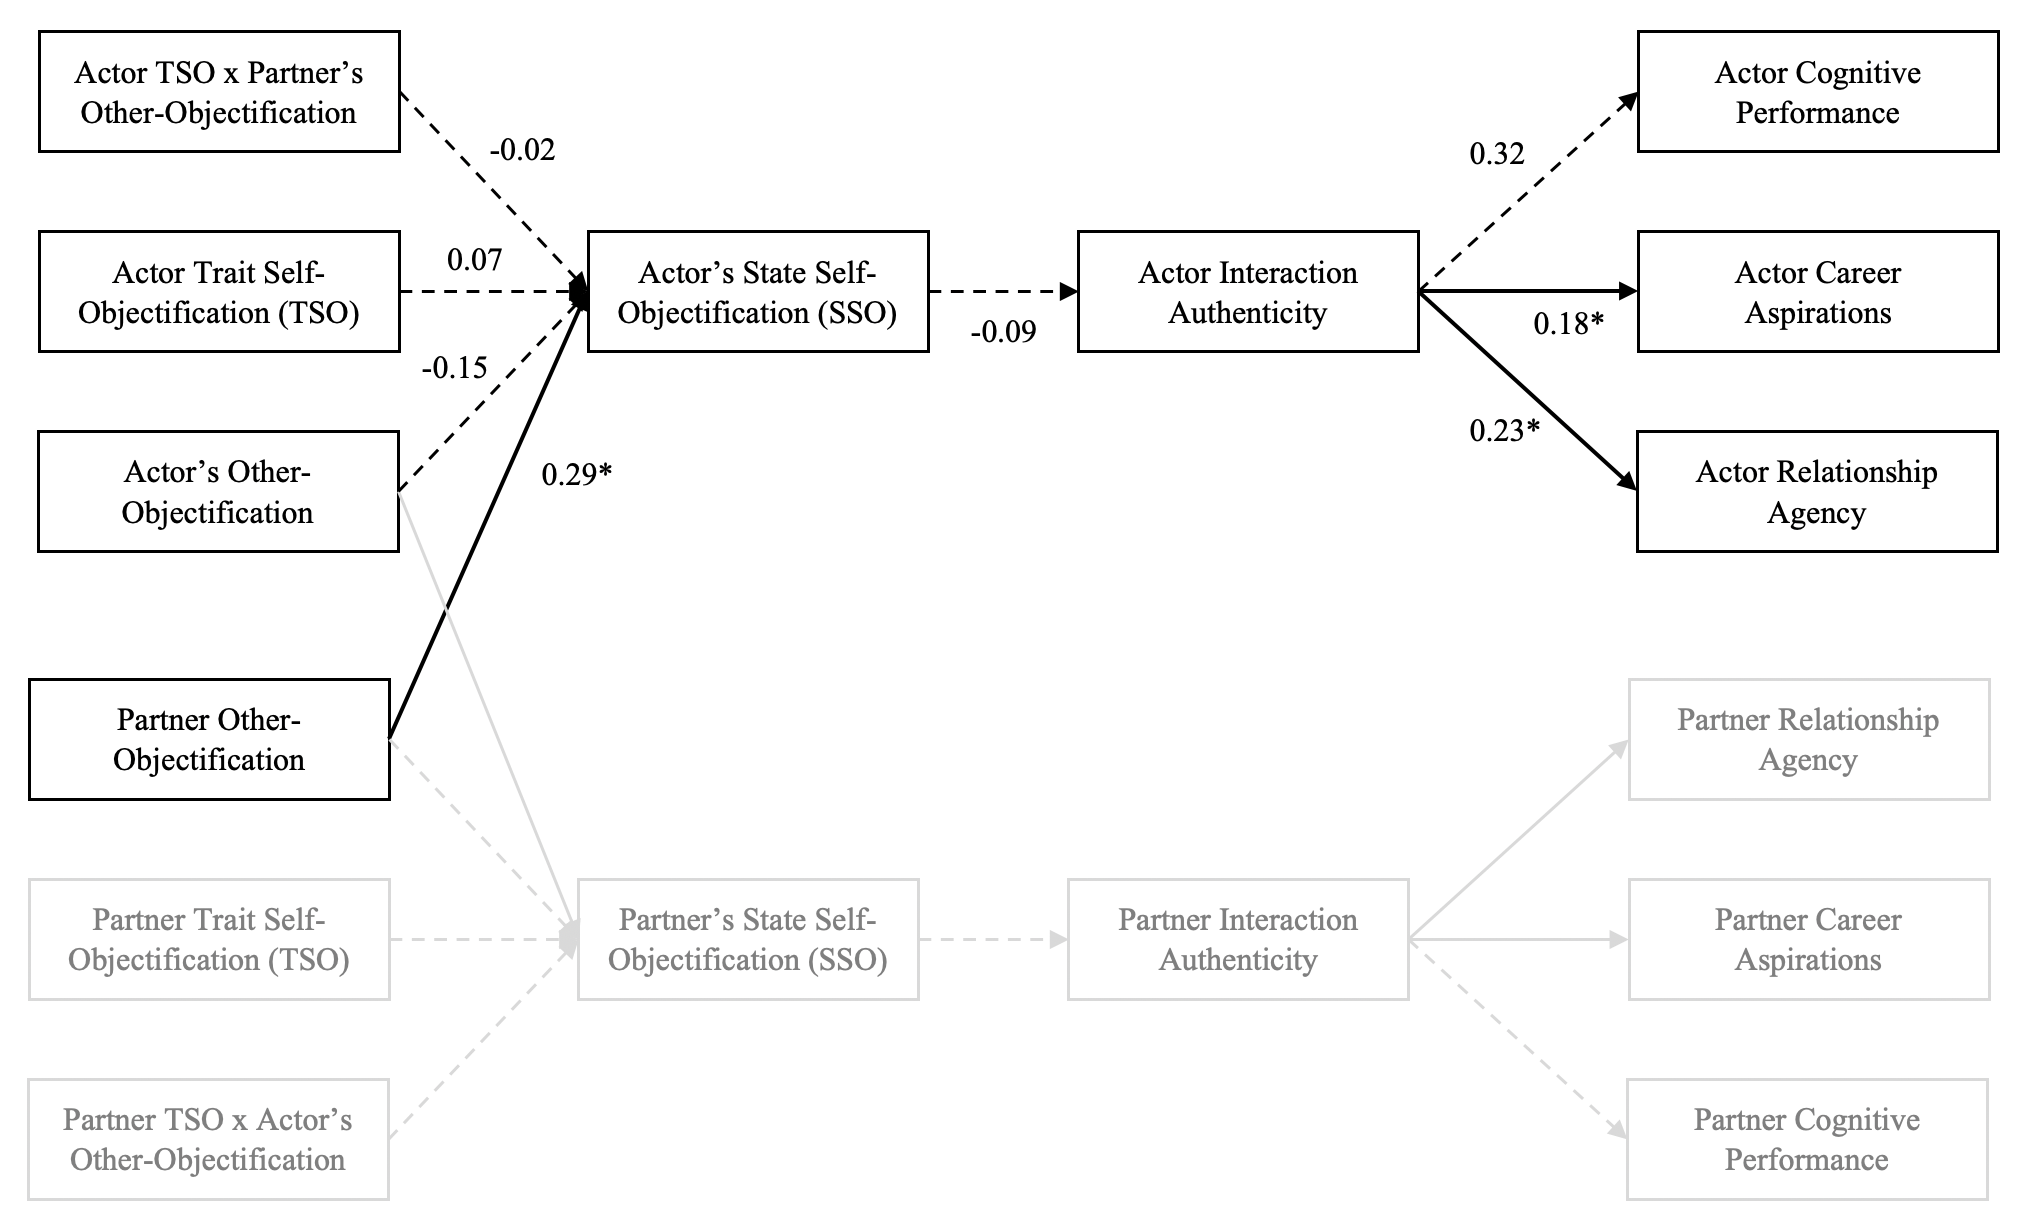
\includegraphics[width=400px]{SEMfigure} \caption{Path Analysis Model with Estimates}\label{fig:semfigure}
\end{figure}

All model estimates and p-values are found in Table~\ref{tab:mlm} and
the relationships with estimates included are depicted in
Figure~\ref{fig:semfigure}.

The most important finding from Garcia et al. (2016) was the significant
partner effect of other objectification and SSO (specifically men's
objectification of women and women's SSO). As expected, the partner
effect of other-objectification on SSO in the current all-women sample
was statistically signficant, \emph{b} = 0.29, \emph{SE} = 0.12,
\emph{p} = .019, replicating Garcia et al. (2016)'s fiding. One's own
other objectification had no effect on SSO, \emph{b} = -0.16, \emph{SE}
= 0.12, \emph{p} = .210. Contrary to past finding however, there was no
statistically significant interaction of partner's other objectification
and the person's trait self-objectification on SSO, \emph{b} = 0.03,
\emph{SE} = 0.27, \emph{p} = .910. There was also no significant main
effect of trait self-objectification on SSO \emph{b} = 0.07, \emph{SE} =
0.05, \emph{p} = .183.

Contrary to expectations, there was no significant effect of SSO on
interaction authenticity, although the estimate of this effect was in
the hypothesized negative direction, \emph{b} = -0.09, \emph{SE} = 0.12,
\emph{p} = .431. Because authenticity was a composite score of 9 items,
two of which were interaction specific authenticity items, we also
estimated the pairwise correlations bewteen SSO and all these items
individually. They were all small, ranging from only -0.01 to -0.14.
Although we hypothesized that SSO would mediate the relationship between
partner's other objectification and interaction authenticity, after
finding no relationship bewteen SSO and authencity, we also tested if
the partner's other objectification had a direct effect on authenticity,
but this effect was not significant, \emph{b} = 0.06, \emph{SE} = 0.12,
\emph{p} = .608 (nor was the total effect of partner's other
objectification on authenticity, \emph{b} = 0.03, \emph{SE} = 0.11,
\emph{p} = .787).

Lastly, althought there was no evidence that SSO was related to
interaction authenticity in the current sample, we tested if interaction
authenticity (composite of nine items) had effects on cognitive
performace, career aspirations, and relationship agency, as it did in
Garcia et al. (2016). We again used MLM and thus, these efefcts were
tested in three separate models. There was no significant effect of
interaction authenticity on cognitive performance, \emph{b} = 0.32,
\emph{SE} = 0.28, \emph{p} = .258, but authenticity was significantly
positively related to both career aspirations, \emph{b} = 0.18,
\emph{SE} = 0.07, \emph{p} = .010, and relationships agency, \emph{b} =
0.23, \emph{SE} = 0.12, \emph{p} = .049. There was no direct effect of
SSO on cognitive performance, \emph{b} = 0.04, \emph{SE} = 0.25,
\emph{p} = .872, and no direct effect of partner's other objectificaiton
on cognifitve performance, \emph{b} = 0.01, \emph{SE} = 0.27, \emph{p} =
.962. There was no direct effect of SSO on career aspirations, \emph{b}
= 0.03, \emph{SE} = 0.06, \emph{p} = .657, and no direct effect of
partner's other objectificaiton on career aspirations, \emph{b} = -0.06,
\emph{SE} = 0.07, \emph{p} = .378. There was no direct effect of SSO on
relationship agency, \emph{b} = -0.05, \emph{SE} = 0.11, \emph{p} =
.659, and no direct effect of partner's other objectificaiton on
relationship agency, \emph{b} = -0.1, \emph{SE} = 0.11, \emph{p} = .365.

The results were similar for analyses conducted on Sample 1 and Sample 2
individually. See the online supplemental material for more detail on
these analyses.

\section{Discussion}\label{discussion}

As stated previously, we did not find a significant effect between actor
SSO and actor authenticity (\(\beta\)= -.10, \(p\)=.38), which suggests
that there is not sufficient evidence to support the claim that partner
objectification is the cause for the diverse range of negative effects
related to relationship inauthenticity. However, we did observe a
significant partner effect of objectification on actor
self-objectification, which does align with our hypothesis that
theorized objectification from other women can also cause women to
self-objectify just as they do within interactions between male-female
pairs. The results of this study demonstrate the complex and ambivalent
nature of female sexual objectification and additionally highlight the
psychological and social consequences of such objectification processes
on women's social relationships and well-being. The sample of the
current study was comprised of Western women, being that sexual
objectification is most prevalent in this culture (Loughnan et al.,
2015), and research on objectification conducted outside of Western or
Westernized countries is scarce (Moradi \& Huang, 2008). Because
\enquote{bodies exist within social and cultural contexts, and hence are
also constructed through sociocultural practices and discourses}
(Roberts \& Fredrickson, 1997, p. 174), it is important to consider how
diverse social identities within unique cultural contexts may inform
sexual objectification phenomenon to test the cross-cultural
applicability of theoretical frameworks (Loughnan et al., 2015).
Further, sexualzing experiences and self-objectification are thought to
begin a very young age, and thus, researchers have only recently begun
to examine such experiences among children (Bury, Tiggemann, \& Slater,
2016; e.g., Holland \& Haslam, 2016; Jongenelis, Byrne, \& Pettigrew,
2014). Considering the fact that the average mean age of the
investigated participants of this current study was 18.85 years,
research among younger and older individuals is needed, especially
because self-objectification may change over time (Roberts \&
Fredrickson, 1997). It may be valuable to question the extent to which
children, adolescents, or emerging adults of different races or
ethnicities are exposed to varied amounts of sexulizing content. Also,
future experiments or longitudinal studies should explore the external
validity of the notions of self-objectification and how the
operalization of self-objectification may be improved. Regardless, the
results from the current analysis highlight how subtle forms of sexist
discrimination operate to inform prevention and intervention efforts in
both clinical and educational contexts. These results are quite useful
for promoting mental health and within early action programs for girls
and young women, where scholars and practitioners might provide the
tools necessary to circumvent or mitigate negative effects on
self-objectification, and combat such experiences.

\section{References}\label{references}

\newpage

\begingroup
\setlength{\parindent}{-0.5in} \setlength{\leftskip}{0.5in}

\hypertarget{refs}{}
\hypertarget{ref-argyle1969}{}
Argyle, M., \& Williams, M. (1969). Observer or observed? A reversible
perspective in person perception. \emph{Sociometry}, 396--412.

\hypertarget{ref-R-papaja}{}
Aust, F., \& Barth, M. (2018). \emph{papaja: Create APA manuscripts with
R Markdown}. Retrieved from \url{https://github.com/crsh/papaja}

\hypertarget{ref-Bartky}{}
Bartky, S. L. (1990). Femininity and domination studies in the
phenomenology of oppression.

\hypertarget{ref-R-Matrix}{}
Bates, D., \& Maechler, M. (2017). \emph{Matrix: Sparse and dense matrix
classes and methods}. Retrieved from
\url{https://CRAN.R-project.org/package=Matrix}

\hypertarget{ref-berger1972}{}
Berger, J., Cohen, B. P., \& Zelditch Jr, M. (1972). Status
characteristics and social interaction. \emph{American Sociological
Review}, 241--255.

\hypertarget{ref-R-lpSolve}{}
Berkelaar, M., \& others. (2015). \emph{LpSolve: Interface to
'lp\_solve' v. 5.5 to solve linear/integer programs}. Retrieved from
\url{https://CRAN.R-project.org/package=lpSolve}

\hypertarget{ref-briton1995}{}
Briton, N. J., \& Hall, J. A. (1995). Beliefs about female and male
nonverbal communication. \emph{Sex Roles}, \emph{32}(1-2), 79--90.

\hypertarget{ref-brunelletal2010}{}
Brunell, A. B., Kernis, M. H., Goldman, B. M., Heppner, W., Davis, P.,
Cascio, E. V., \& Webster, G. D. (2010). Dispositional authenticity and
romantic relationship functioning. \emph{Personality and Individual
Differences}, \emph{48}(8), 900--905.
doi:\href{https://doi.org/10.1016/j.paid.2010.02.018}{10.1016/j.paid.2010.02.018}

\hypertarget{ref-bury2016}{}
Bury, B., Tiggemann, M., \& Slater, A. (2016). Disclaimer labels on
fashion magazine advertisements: Impact on visual attention and
relationship with body dissatisfaction. \emph{Body Image}, \emph{16},
1--9.

\hypertarget{ref-calogero2011}{}
Calogero, R. M., Tantleff-Dunn, S. E., \& Thompson, J. (2011).
\emph{Self-objectification in women: Causes, consequences, and
counteractions.} American Psychological Association.

\hypertarget{ref-R-xtable}{}
Dahl, D. B., Scott, D., Roosen, C., Magnusson, A., \& Swinton, J.
(2019). \emph{Xtable: Export tables to latex or html}. Retrieved from
\url{https://CRAN.R-project.org/package=xtable}

\hypertarget{ref-Kaschak}{}
Engendered lives: A new psychology of womens experience. (1993).
\emph{Choice Reviews Online}, \emph{30}(07).
doi:\href{https://doi.org/10.5860/choice.30-4102}{10.5860/choice.30-4102}

\hypertarget{ref-frasernicholson1989}{}
Fraser, N., \& Nicholson, L. (1989). Social criticism without
philosophy: An encounter between feminism and postmodernism.
\emph{Social Text}, (21), 83.
doi:\href{https://doi.org/10.2307/827810}{10.2307/827810}

\hypertarget{ref-fredricksonetal2011}{}
Fredrickson, B. L., Hendler, L. M., Nilsen, S., O'Barr, J. F., \&
Roberts, T.-A. (2011). Bringing back the body. \emph{Psychology of Women
Quarterly}, \emph{35}(4), 689--696.
doi:\href{https://doi.org/10.1177/0361684311426690}{10.1177/0361684311426690}

\hypertarget{ref-R-irr}{}
Gamer, M., Lemon, J., \&
\textless{}puspendra.pusp22@gmail.com\textgreater{}, I. F. P. S. (2012).
\emph{Irr: Various coefficients of interrater reliability and
agreement}. Retrieved from \url{https://CRAN.R-project.org/package=irr}

\hypertarget{ref-garcia2016objectification}{}
Garcia, R. L., Earnshaw, V. A., \& Quinn, D. M. (2016). Objectification
in action: Self-and other-objectification in mixed-sex interpersonal
interactions. \emph{Psychology of Women Quarterly}, \emph{40}(2),
213--228.

\hypertarget{ref-garcia2015moderation}{}
Garcia, R. L., Kenny, D. A., \& Ledermann, T. (2015). Moderation in the
actor--partner interdependence model. \emph{Personal Relationships},
\emph{22}(1), 8--29.

\hypertarget{ref-R-purrr}{}
Henry, L., \& Wickham, H. (2019). \emph{Purrr: Functional programming
tools}. Retrieved from \url{https://CRAN.R-project.org/package=purrr}

\hypertarget{ref-holland2016}{}
Holland, E., \& Haslam, N. (2016). Cute little things: The
objectification of prepubescent girls. \emph{Psychology of Women
Quarterly}, \emph{40}(1), 108--119.

\hypertarget{ref-R-kutils}{}
Johnson, P., Kite, B., \& Redmon, C. (2019). \emph{Kutils: Project
management tools}. Retrieved from
\url{https://CRAN.R-project.org/package=kutils}

\hypertarget{ref-jongenelis2014}{}
Jongenelis, M. I., Byrne, S. M., \& Pettigrew, S. (2014).
Self-objectification, body image disturbance, and eating disorder
symptoms in young australian children. \emph{Body Image}, \emph{11}(3),
290--302.

\hypertarget{ref-R-ggformula}{}
Kaplan, D., \& Pruim, R. (2017). \emph{Ggformula: Formula interface to
the grammar of graphics}. Retrieved from
\url{https://CRAN.R-project.org/package=ggformula}

\hypertarget{ref-fredricksonetal1998}{}
L. Fredrickson, B., Roberts, T.-A., M. Noll, S., Quinn, D., \& Twenge,
J. (1998). That swimsuit becomes you: Sex differences in
self-objedification, restrained eating, and math performance.
\emph{Journal of Personality and Social Psychology}, \emph{75}, 269--84.
doi:\href{https://doi.org/10.1037/0022-3514.75.1.269}{10.1037/0022-3514.75.1.269}

\hypertarget{ref-ledermann2017analyzing}{}
Ledermann, T., \& Kenny, D. A. (2017). Analyzing dyadic data with
multilevel modeling versus structural equation modeling: A tale of two
methods. \emph{Journal of Family Psychology}, \emph{31}(4), 442.

\hypertarget{ref-loughnan2015}{}
Loughnan, S., Fernandez-Campos, S., Vaes, J., Anjum, G., Aziz, M.,
Harada, C., \ldots{} Tsuchiya, K. (2015). Exploring the role of culture
in sexual objectification: A seven nations study. \emph{Revue
Internationale de Psychologie Sociale}, \emph{28}(1), 125--152.

\hypertarget{ref-nollfredrickson1998}{}
M. Noll, S., \& L. Fredrickson, B. (1998). A mediational model linking
self-objectification, body shame, and disordered eating.
\emph{Psychology of Women Quarterly}, \emph{22}, 623--636.
doi:\href{https://doi.org/10.1111/j.1471-6402.1998.tb00181.x}{10.1111/j.1471-6402.1998.tb00181.x}

\hypertarget{ref-mcfarlin1984remote}{}
McFarlin, D. B., \& Blascovich, J. (1984). On the remote associates test
(rat) as an alternative to illusory performance feedback: A
methodological note. \emph{Basic and Applied Social Psychology},
\emph{5}(3), 223--229.

\hypertarget{ref-moradi2008}{}
Moradi, B., \& Huang, Y.-P. (2008). Objectification theory and
psychology of women: A decade of advances and future directions.
\emph{Psychology of Women Quarterly}, \emph{32}(4), 377--398.

\hypertarget{ref-R-tibble}{}
Müller, K., \& Wickham, H. (2019). \emph{Tibble: Simple data frames}.
Retrieved from \url{https://CRAN.R-project.org/package=tibble}

\hypertarget{ref-olsen2006structural}{}
Olsen, J. A., \& Kenny, D. A. (2006). Structural equation modeling with
interchangeable dyads. \emph{Psychological Methods}, \emph{11}(2), 127.

\hypertarget{ref-grayobrien2007}{}
P. Gray, M., \& M. OBrien, K. (2007). Advancing the assessment of
women's career choices: The career aspiration scale. \emph{Journal of
Career Assessment - J CAREER ASSESSMENT}, \emph{15}, 317--337.
doi:\href{https://doi.org/10.1177/1069072707301211}{10.1177/1069072707301211}

\hypertarget{ref-R-nlme}{}
Pinheiro, J., Bates, D., DebRoy, S., Sarkar, D., \& R Core Team. (2017).
\emph{nlme: Linear and nonlinear mixed effects models}. Retrieved from
\url{https://CRAN.R-project.org/package=nlme}

\hypertarget{ref-R-mosaic}{}
Pruim, R., Kaplan, D. T., \& Horton, N. J. (2017). The mosaic package:
Helping students to 'think with data' using r. \emph{The R Journal},
\emph{9}(1), 77--102. Retrieved from
\url{https://journal.r-project.org/archive/2017/RJ-2017-024/index.html}

\hypertarget{ref-R-mosaicData}{}
Pruim, R., Kaplan, D., \& Horton, N. (2016). \emph{MosaicData: Project
mosaic data sets}. Retrieved from
\url{https://CRAN.R-project.org/package=mosaicData}

\hypertarget{ref-quinnetal}{}
Quinn, D. M., Chaudoir, S. R., \& Kallen, R. W. (2011). Performance and
flow: A review and integration of self-objectification research.
\emph{Self-Objectification in Women: Causes, Consequences, and
Counteractions.}, 119--138.
doi:\href{https://doi.org/10.1037/12304-006}{10.1037/12304-006}

\hypertarget{ref-R-base}{}
R Core Team. (2017). \emph{R: A language and environment for statistical
computing}. Vienna, Austria: R Foundation for Statistical Computing.
Retrieved from \url{https://www.R-project.org/}

\hypertarget{ref-R-psych}{}
Revelle, W. (2017). \emph{Psych: Procedures for psychological,
psychometric, and personality research}. Evanston, Illinois:
Northwestern University. Retrieved from
\url{https://CRAN.R-project.org/package=psych}

\hypertarget{ref-robertsfredrickson}{}
Roberts, T.-A., \& Fredrickson, B. L. (1997). Objectification theory.
\emph{Encyclopedia of Social Psychology}.
doi:\href{https://doi.org/10.4135/9781412956253.n377}{10.4135/9781412956253.n377}

\hypertarget{ref-R-lavaan}{}
Rosseel, Y. (2012). lavaan: An R package for structural equation
modeling. \emph{Journal of Statistical Software}, \emph{48}(2), 1--36.
Retrieved from \url{http://www.jstatsoft.org/v48/i02/}

\hypertarget{ref-rubin1975}{}
Rubin, J. (1975). What the ``good language learner'' can teach us.
\emph{TESOL Quarterly}, \emph{9}(1), 41.
doi:\href{https://doi.org/10.2307/3586011}{10.2307/3586011}

\hypertarget{ref-saguyetal2010}{}
Saguy, T., Quinn, D., F Dovidio, J., \& Pratto, F. (2010). Interacting
like a body: Objectification can lead women to narrow their presence in
social interactions. \emph{Psychological Science}, \emph{21}, 178--82.
doi:\href{https://doi.org/10.1177/0956797609357751}{10.1177/0956797609357751}

\hypertarget{ref-R-lattice}{}
Sarkar, D. (2008). \emph{Lattice: Multivariate data visualization with
r}. New York: Springer. Retrieved from
\url{http://lmdvr.r-forge.r-project.org}

\hypertarget{ref-R-apaTables}{}
Stanley, D. (2018). \emph{ApaTables: Create american psychological
association (apa) style tables}. Retrieved from
\url{https://CRAN.R-project.org/package=apaTables}

\hypertarget{ref-swimetal}{}
Swim, J. K., Hyers, L. L., Cohen, L. L., \& Ferguson, M. J. (2001).
Everyday sexism: Evidence for its incidence, nature, and psychological
impact from three daily diary studies. \emph{Journal of Social Issues},
\emph{57}(1), 31--53.
doi:\href{https://doi.org/10.1111/0022-4537.00200}{10.1111/0022-4537.00200}

\hypertarget{ref-R-ggplot2}{}
Wickham, H. (2016). \emph{Ggplot2: Elegant graphics for data analysis}.
Springer-Verlag New York. Retrieved from
\url{https://ggplot2.tidyverse.org}

\hypertarget{ref-R-tidyverse}{}
Wickham, H. (2017). \emph{Tidyverse: Easily install and load the
'tidyverse'}. Retrieved from
\url{https://CRAN.R-project.org/package=tidyverse}

\hypertarget{ref-R-forcats}{}
Wickham, H. (2018). \emph{Forcats: Tools for working with categorical
variables (factors)}. Retrieved from
\url{https://CRAN.R-project.org/package=forcats}

\hypertarget{ref-R-stringr}{}
Wickham, H. (2019). \emph{Stringr: Simple, consistent wrappers for
common string operations}. Retrieved from
\url{https://CRAN.R-project.org/package=stringr}

\hypertarget{ref-R-usethis}{}
Wickham, H., \& Bryan, J. (2018). \emph{Usethis: Automate package and
project setup}. Retrieved from
\url{https://CRAN.R-project.org/package=usethis}

\hypertarget{ref-R-tidyr}{}
Wickham, H., \& Henry, L. (2019). \emph{Tidyr: Easily tidy data with
'spread()' and 'gather()' functions}. Retrieved from
\url{https://CRAN.R-project.org/package=tidyr}

\hypertarget{ref-R-haven}{}
Wickham, H., \& Miller, E. (2019). \emph{Haven: Import and export
'spss', 'stata' and 'sas' files}. Retrieved from
\url{https://CRAN.R-project.org/package=haven}

\hypertarget{ref-R-dplyr}{}
Wickham, H., François, R., Henry, L., \& Müller, K. (2018). \emph{Dplyr:
A grammar of data manipulation}. Retrieved from
\url{https://CRAN.R-project.org/package=dplyr}

\hypertarget{ref-R-devtools}{}
Wickham, H., Hester, J., \& Chang, W. (2018). \emph{Devtools: Tools to
make developing r packages easier}. Retrieved from
\url{https://CRAN.R-project.org/package=devtools}

\hypertarget{ref-R-readr}{}
Wickham, H., Hester, J., \& Francois, R. (2017). \emph{Readr: Read
rectangular text data}. Retrieved from
\url{https://CRAN.R-project.org/package=readr}

\hypertarget{ref-R-knitr}{}
Xie, Y. (2015). \emph{Dynamic documents with R and knitr} (2nd ed.).
Boca Raton, Florida: Chapman; Hall/CRC. Retrieved from
\url{https://yihui.name/knitr/}

\hypertarget{ref-young1979}{}
Young, I. M. (1979). \emph{Proceedings of the second sex---Thirty years
later: A commemorative conference on feminist theory,}

\endgroup


\end{document}
